
%----------------------------------------------------------------------------------------
%	PACKAGES AND OTHER DOCUMENT CONFIGURATIONS
%----------------------------------------------------------------------------------------

\documentclass[final]{beamer}

\usepackage[scale=1.24]{beamerposter} % Use the beamerposter package for laying out the poster
%\usetheme{confposter} % Use the confposter theme supplied with this template
\usepackage{amsmath}
\usepackage{amssymb}
\usepackage{mathptmx}
\usetheme[faculty=phil]{fibeamer}
\usefonttheme[onlymath]{serif}

\newlength{\sepwid}
\newlength{\onecolwid}
\newlength{\sidewid}
\newlength{\midwid}
\newlength{\twocolwid}
\newlength{\threecolwid}
\setlength{\paperwidth}{46.8in} % A0 width: 46.8in
\setlength{\paperheight}{33.1in} % A0 height: 33.1in
\setlength{\sepwid}{0.02\paperwidth} % Separation width (white space) between columns
\setlength{\onecolwid}{0.21\paperwidth} % Width of one column
\setlength{\sidewid}{0.19\paperwidth}
\setlength{\midwid}{0.26\paperwidth}

\setlength{\twocolwid}{0.54\paperwidth} % Width of two columns
\setlength{\threecolwid}{0.678\paperwidth} % Width of three columns
%\setlength{\topmargin}{-0.5in} % Reduce the top margin size
%-----------------------------------------------------------

\usepackage{graphicx}  % Required for including images

\usepackage{booktabs} % Top and bottom rules for tables

%----------------------------------------------------------------------------------------
%	TITLE SECTION 
%----------------------------------------------------------------------------------------

\title{Belief Distribution Learning} % Poster title

\author{Duncan Cameron-Steinke} % Author(s)

\institute{The University of British Columbia, Okanagan Campus - June 2, 2026} % Institution(s)

%----------------------------------------------------------------------------------------

\begin{document}
\addtobeamertemplate{block end}{}{\vspace*{2ex}} % White space under blocks
\addtobeamertemplate{block example end}{}{\vspace*{2ex}} % White space under example blocks
\addtobeamertemplate{block alerted end}{}{\vspace*{2ex}} % White space under highlighted (alert) blocks

\setlength{\belowcaptionskip}{2ex} % White space under figures
\setlength\belowdisplayshortskip{2ex} % White space under equations
%\begin{darkframes} % Uncomment for dark theme, don't forget to \end{darkframes}
\begin{frame} % The whole poster is enclosed in one beamer frame

%==========================Begin Head===============================

\begin{columns}
  \begin{column}{0.25\linewidth}
    \centering
    
\includegraphics[width=0.8\linewidth]{img/ubc_logo.png}
  \end{column}

  \begin{column}{0.5\linewidth}
    \vskip1cm
    \centering
    \usebeamercolor{title in headline}{\color{fg}\Huge{\textbf{\inserttitle}}\\[0.5ex]}
    \usebeamercolor{author in headline}{\color{fg}\Large{\insertauthor}\\[1ex]}
    \usebeamercolor{institute in headline}{\color{fg}\large{\insertinstitute}\\[1ex]}
    \vskip1cm
  \end{column}

  \begin{column}{0.25\linewidth}
    \centering
    
\includegraphics[width=0.8\linewidth]{img/CSSC logo.jpg}
  \end{column}
\end{columns}
\vspace{1cm}

%==========================End Head===============================

\begin{columns}[t] % The whole poster consists of three major columns, the second of which is split into two columns twice - the [t] option aligns each column's content to the top

\begin{column}{\sepwid}\end{column} % Empty spacer column

\begin{column}{\sidewid} % The first column

%----------------------------------------------------------------------------------------
%	OBJECTIVES
%----------------------------------------------------------------------------------------

\begin{exampleblock}{Research Objective}
Model label distributions with accurate predictions and well-calibrated uncertainty.

\end{exampleblock}

%----------------------------------------------------------------------------------------
%	INTRODUCTION
%----------------------------------------------------------------------------------------

\begin{exampleblock}{Background}
\textbf{Label Distribution Learning} (LDL) predicts a probability distribution 
over labels for each sample — e.g., predicting that a dog is 75\% Golden Retriever and 25\% 
Poodle.
\vspace{1em}

\textbf{Dirichlet Distribution}
is a probability distribution on the K-dimensional simplex with parameters $\boldsymbol{\alpha}$ representing evidence toward each label:
\begin{equation*}
    \text{Dir}(\mathbf{p} \mid \boldsymbol{\alpha}) = \frac{1}{B(\boldsymbol{\alpha})}\prod_{i=1}^K p_i^{\alpha_i - 1}
\end{equation*}
where $B(\boldsymbol{\alpha})$ is the multinomial Beta function.
Dirichlet can be used in LDL to obtain point estimates with uncertainty.\\
\vspace{1em}
\textbf{Beta distribution} is a special case of Dirichlet when $K = 2$.
\vspace{1em}
\end{exampleblock}
\begin{exampleblock}{Evidential Deep Learning} 
In EDL \cite{sensoy_evidential_2018}, a neural network predicts positive evidence vectors for each label using a ReLU output which directly parameterize a Dirichlet distribution
\begin{equation*}
    \boldsymbol{\alpha} = f_{\theta}(X)+\boldsymbol{1} \quad (\text{ReLU)}
\end{equation*}
where $f_{\theta}(X)$ are the neural network predictions for input $X$ and learned parameters $\hat\theta$.\\
\textbf{The Problem:} Each parameter is independent, violating LDL principles.
\end{exampleblock}
%------------------------------------------------


%----------------------------------------------------------------------------------------

\end{column} % End of the first column

\begin{column}{\sepwid}\end{column} % Empty spacer column

\begin{column}{\twocolwid} % Begin a column which is two columns wide (column 2)

\begin{columns}[t,totalwidth=\twocolwid] % Split up the two columns wide column

\begin{column}{\midwid}\vspace{-.74in} % The first column within column 2 (column 2.1)

%----------------------------------------------------------------------------------------
%	MATERIALS
%----------------------------------------------------------------------------------------

\begin{exampleblock}{Belief Distribution Learning (ours)}
In BDL, a probability estimate $\mathbf{p}$ is decomposed into three components: belief mass $\mathbf{b}$, uncertainty mass $u$, and prior probability $\boldsymbol{a}$ \cite{josang_subjective_2016}:
\begin{align*}
    \mathbf{p} &= \mathbf{b} + u\boldsymbol{a} \\
    1 &= u + \sum \mathbf{b}.
\end{align*}
A neural network with learned parameters $\hat\theta$ predicts the belief vector and uncertainty scalar using a Softmax output,
\begin{equation*}
    u, \mathbf{b} = f_\theta(X) \quad (\text{Softmax}),
\end{equation*}
which parametrize a Dirichlet distribution using
\begin{equation*}
    \boldsymbol{\alpha} = \frac{1}{K}\left(\frac{\mathbf{b}}{u} + \mathbf{a}\right) + 1.
\end{equation*}
\end{exampleblock}

\begin{exampleblock}{multi-Belief Distribution Learning (ours)}
In mBDL, uncertainty is instead predicted per label
\begin{equation*}
    \mathbf{u}, \mathbf{b} = f_\theta(X) \quad (\text{Softmax}).
\end{equation*}

\begin{center}
    \textbf{Sample mBDL Prediction}
\end{center}
\begin{figure}
    \centering
    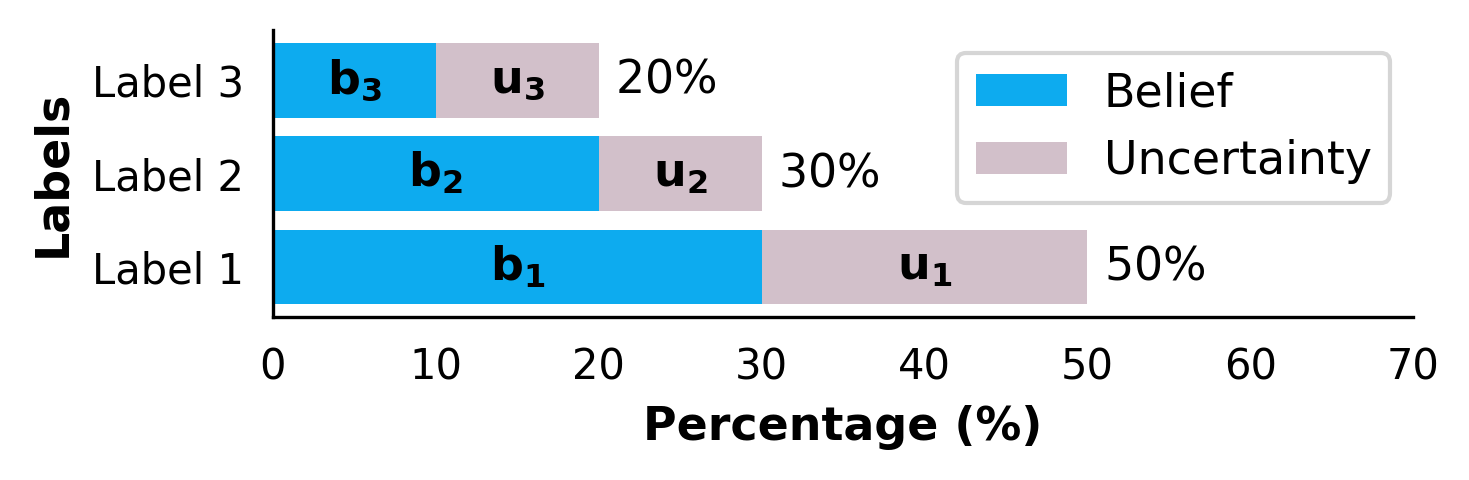
\includegraphics[width=0.9\linewidth]{img/sample_mBDL.png}
\end{figure}
The probability estimate is
\begin{equation*}
    \textbf{p}=\textbf{b}+\textbf{u}.
\end{equation*}
Uncertainty per label is a \textbf{one-vs-rest} Beta distribution:
\begin{align*}
    \text{one:} \quad \alpha_i &= \frac{1}{K}\!\left(\frac{b_i + u_i}{u_i}\right) + 1\\
    \text{rest:} \quad \beta_i &= \frac{1}{K}\!\left(\frac{1 - (b_i + u_i)}{u_i}\right) + 1
\end{align*}

The joint PDF is the product over all labels:
\vspace{-0.5em}
\begin{equation}
    \text{mBDL}(\mathbf{p} \mid \boldsymbol{\alpha}, \boldsymbol{\beta})
    = \prod_{i=1}^K \text{Beta}(p_i \mid \alpha_i, \beta_i)
\end{equation}


\end{exampleblock}


%----------------------------------------------------------------------------------------

\end{column} % End of column 2.1
\begin{column}{\sepwid}\end{column} % Empty spacer column

\begin{column}{\midwid}\vspace{-.74in} % The second column within column 2 (column 2.2)

%----------------------------------------------------------------------------------------
%	METHODS
%----------------------------------------------------------------------------------------
\begin{exampleblock}{Benefit of Belief Logic}
    Belief logic enforces the simplex constraint. Unlike with evidence vectors, increasing belief in one label \textit{requires} reducing belief in others, which directly aligns with LDL.
\end{exampleblock}

\begin{exampleblock}{Results}

\begin{center}
    \textbf{Uncertainty Distributions}
\end{center}
    \begin{figure}
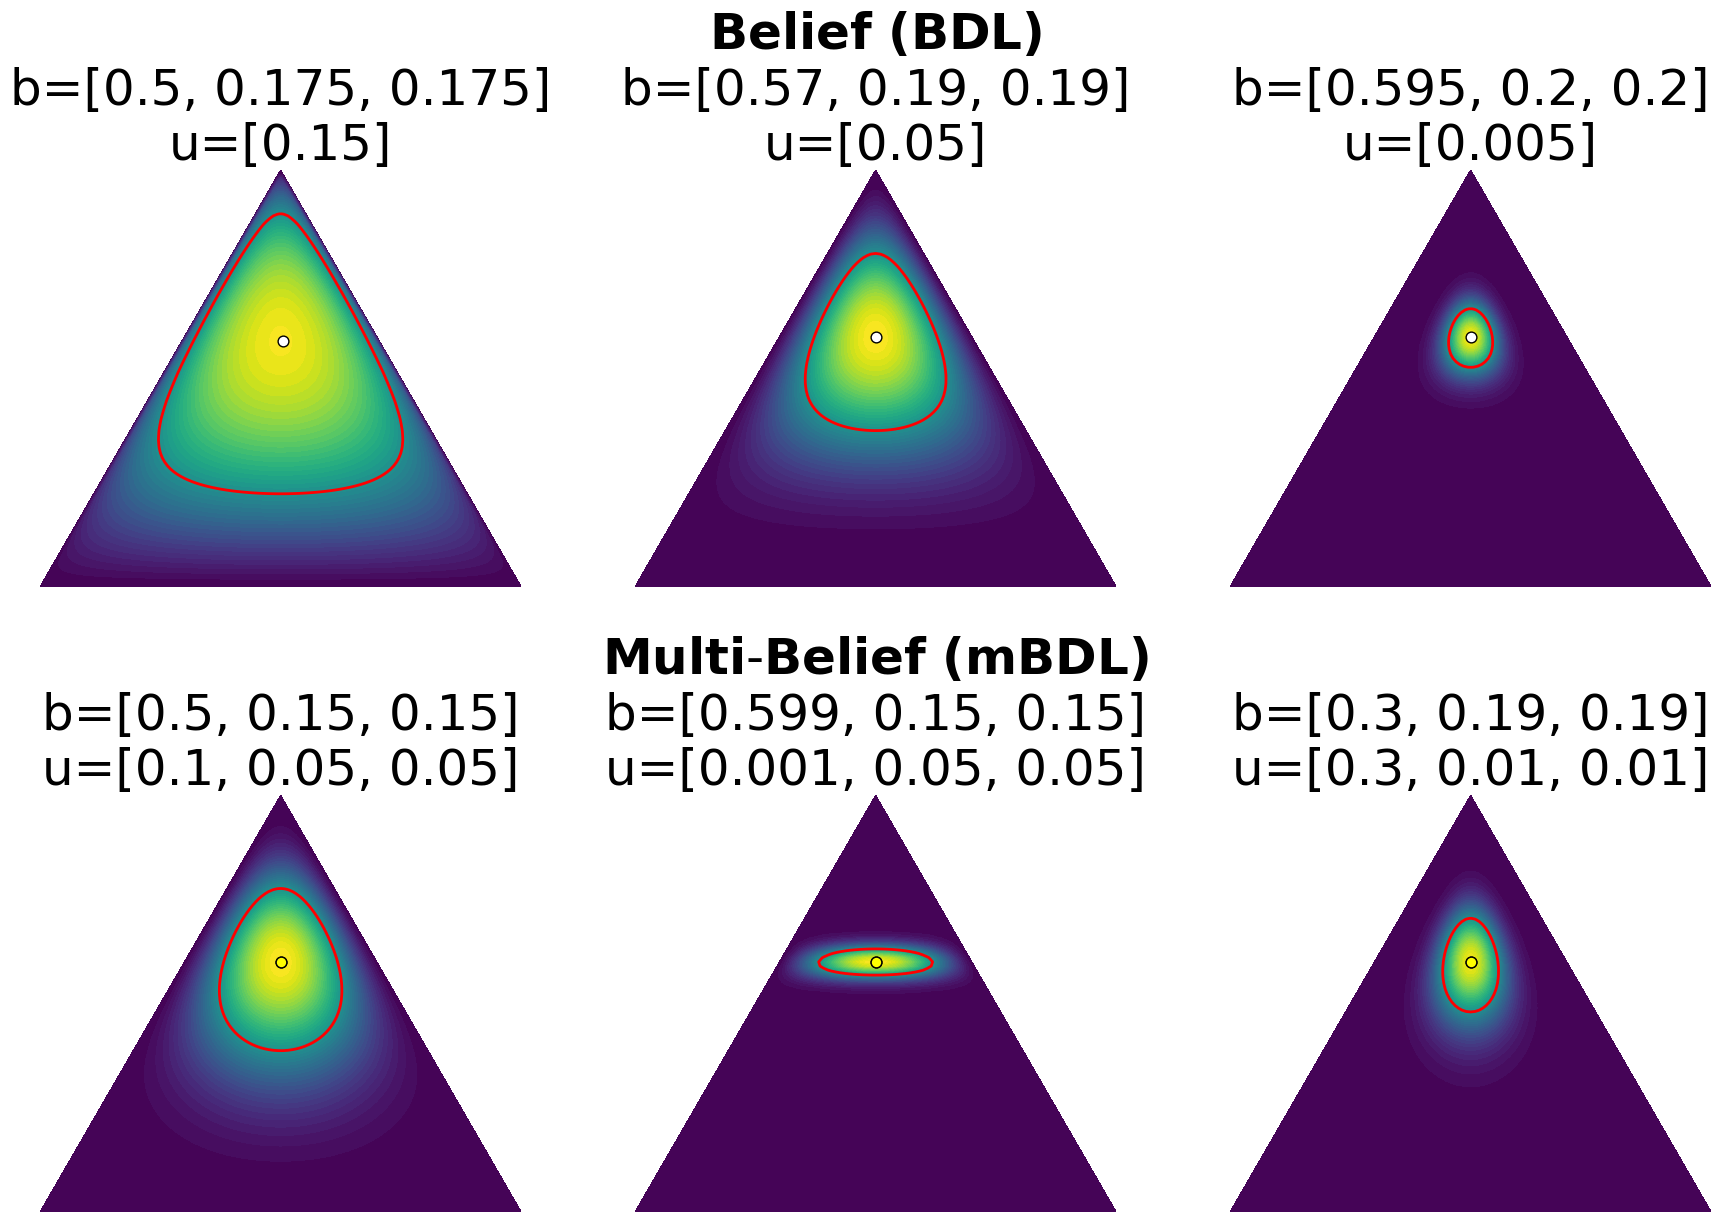
\includegraphics[width=1\linewidth]{img/bdl_mbdl.png}
\end{figure}
\footnotesize
Uncertainty distributions for BDL (top), and mBDL (bottom) under various parameters. The white dot is the prediction. Red contours show 50\% credible region. \\
\normalsize
\vspace{1em}
EDL (not shown) and BDL both produce symmetric Dirichlet distributions which restrict their flexibility. mBDL allows for asymmetry, providing better calibrated uncertainty.
\vspace{0.5em}

\begin{center}
    \textbf{Accuracy and Calibration Results}
\end{center}
   \begin{table}
        \centering

        \begin{tabular}{lccc}
            \toprule
            \textbf{Model} & \textbf{KL Div.} $\downarrow$ & \textbf{Joint FSC} $\uparrow$ & \textbf{Worst-Bin FSC} $\uparrow$ \\
            \midrule
            BDL              & \textbf{0.042}$\pm$0.003 & 0.55$\pm$0.03 & 0.52$\pm$0.04 \\
            \textbf{mBDL} & \textbf{0.042}$\pm$0.002 & \textbf{0.59}$\pm$0.04 & \textbf{0.57}$\pm$0.03 \\
            EDL              & 0.060$\pm$0.005 & 0.51$\pm$0.03 & 0.49$\pm$0.02 \\
            DP               & 0.073$\pm$0.004 & 0.50$\pm$0.04 & 0.55$\pm$0.03 \\
            SNEFY            & 0.141$\pm$0.013 & 0.57$\pm$0.04 & 0.54$\pm$0.03 \\
            \bottomrule
        \end{tabular}
    \end{table}
    \footnotesize
    \textbf{BDL} (ours): Belief Distribution Learning \quad \textbf{mBDL} (ours)
multi-Belief Distribution Learning     \textbf{EDL}: Evidential Deep Learning
    \textbf{DP}: Direct Prediction with Bayesian dropout for uncertainty estimates \quad
    \textbf{SNEFY}: Squared Neural Family \cite{zhang_label_2025} \\


\end{exampleblock}

%----------------------------------------------------------------------------------------

\end{column} % End of column 2.2

\end{columns} % End of the split of column 2 - any content after this will now take up 2 columns width

%----------------------------------------------------------------------------------------
%	IMPORTANT RESULT
%----------------------------------------------------------------------------------------

% \begin{exampleblock}{Results}


% %----------------------------------------------------------------------------------------

% \begin{columns}[t,totalwidth=\twocolwid] % Split up the two columns wide column again

% \begin{column}{\midwid} % The first column within column 2 (column 2.1)



% %----------------------------------------------------------------------------------------

% \end{column} % End of column 2.1
% \begin{column}{\sepwid}\end{column} % Empty spacer column

% \begin{column}{\midwid} % The second column within column 2 (column 2.2)

% %----------------------------------------------------------------------------------------

% \end{column} % End of column 2.2

% \end{columns} % End of the split of column 2
% \end{exampleblock} 
\end{column} % End of the second column

\begin{column}{\sepwid}\end{column} % Empty spacer column

\begin{column}{\sidewid} % The third column

%----------------------------------------------------------------------------------------
%	CONCLUSION
%----------------------------------------------------------------------------------------

% \end{figure}
\begin{exampleblock}{Conclusion}
    Belief logic improves LDL accuracy and asymmetric distributions improve uncertainty calibration.
\end{exampleblock}
\begin{exampleblock}{Metrics}
\textbf{Kullback-Leibler Divergence} (KL Div.): measure of agreement between two probability vectors.

\textbf{Feature Stratified Coverage} (FSC): Per-label coverage of the 90\% conformal region, based on calibrated conformal intervals. \\
\textbf{Joint FSC}: The 90\% conformal coverage considering all labels simultaneously.\\
\textbf{Worst-Bin FSC}: Each label is split into 4 quartiles, the lowest FSC score across bins and labels is recorded.

\end{exampleblock}



%----------------------------------------------------------------------------------------
%	REFERENCES
%----------------------------------------------------------------------------------------

\begin{exampleblock}{References}

% \nocite{*} % Insert publications even if they are not cited in the poster
\small{\bibliographystyle{ieeetr}
\bibliography{references}}
\end{exampleblock}

%----------------------------------------------------------------------------------------
%	ACKNOWLEDGEMENTS
%----------------------------------------------------------------------------------------

%\setbeamercolor{block title}{fg=red,bg=white} % Change the block title color

%\begin{exampleblock}{Acknowledgements}

%\small{\rmfamily{Nam mollis tristique neque eu luctus. Suspendisse rutrum congue nisi sed convallis. Aenean id neque dolor. Pellentesque habitant morbi tristique senectus et netus et malesuada fames ac turpis egestas.}} \\

%\end{exampleblock}

%----------------------------------------------------------------------------------------
%	CONTACT INFORMATION
%----------------------------------------------------------------------------------------

%\setbeamercolor{block alerted title}{fg=black,bg=norange} % Change the alert block title colors
%\setbeamercolor{block alerted body}{fg=black,bg=white} % Change the alert block body colors

\begin{block}{Contact Information}

\begin{itemize}
\item Email: \href{mailto:dcameronsteinke@gmail.com}{dcameronsteinke@gmail.com}
\end{itemize}

\end{block}


%----------------------------------------------------------------------------------------

\end{column} % End of the third column

\begin{column}{\sepwid}\end{column} % Empty spacer column

\end{columns} % End of all the columns in the poster

\end{frame} % End of the enclosing frame
%\end{darkframes} % Uncomment for dark theme
\end{document}
